\PassOptionsToPackage{unicode}{hyperref}
\documentclass[aspectratio=1610, captions=tableheading, 11pt]{beamer}
\usepackage{booktabs}
% Load packages you need here
\usepackage{polyglossia}
\setmainlanguage{german}

\usepackage{csquotes}

%% Macros for Quote

\def\signed #1{{\leavevmode\unskip\nobreak\hfil\penalty50\hskip1em
  \hbox{}\nobreak\hfill #1%
  \parfillskip=0pt \finalhyphendemerits=0 \endgraf}}

\newsavebox\mybox
\newenvironment{aquote}[1]
  {\savebox\mybox{#1}\begin{quote}}
  {\vspace*{5mm}\signed{\usebox\mybox}\end{quote}}
    
%% \Macros

\usepackage{appendixnumberbeamer} 

\usepackage{caption}
\usepackage{varwidth}
\DeclareCaptionFormat{myformat}{%
  % #1: label (e.g. "Table 1")
  % #2: separator (e.g. ": ")
  % #3: caption text
  \begin{varwidth}{\linewidth}%
    \centering
    #1#2#3%
  \end{varwidth}%
}

\AtBeginSection[]{
  \begin{frame}
  \vfill
  \centering
  \begin{beamercolorbox}[sep=8pt,center,shadow=true,rounded=true]{title}
    \usebeamerfont{title}\insertsectionhead\par%
  \end{beamercolorbox}
  \vfill
  \end{frame}
}

\usepackage{amsmath}
\usepackage{amssymb}
\usepackage{mathtools}
\usepackage[mathrm=sym]{unicode-math}
\usepackage{relsize}
\usepackage{listings}

\usepackage[
  locale=DE,                 % deutsche Einstellungen
  separate-uncertainty=true, % immer Fehler mit \pm
  per-mode=reciprocal,       % ^-1 für inverse Einheiten
  % alternativ:
  % per-mode=reciprocal, % m s^{-1}
  % decimal-marker=., % . statt , f�r Dezimalzahlen
]{siunitx}

\usepackage{hyperref}
\usepackage{bookmark}
\usepackage[utf8]{inputenc}

% load the theme after all packages

\usetheme[
  showtotalframes, % show total number of frames in the footline
]{tudo}

% Put settings here, like
\unimathsetup{
  math-style=ISO,
  bold-style=ISO,
  nabla=upright,
  partial=upright,
  mathrm=sym,
}

\usepackage{tikz-feynman}
\usepackage{xfrac}
\usepackage{tikz}
\usetikzlibrary{shapes,arrows}

\tikzstyle{decision} = [rectangle, draw, fill=tucitron!20, 
    text width=15em, text centered, rounded corners, minimum height=2em]
\tikzstyle{onlytext} = [rectangle, draw=none, 
    text width=15em, text centered, rounded corners, minimum height=2em]
\tikzstyle{block} = [rectangle, draw, fill=tugreen!20, 
    text width=20em, text centered, rounded corners, minimum height=2em]
 \tikzstyle{blockH} = [rectangle, draw, fill=tugreen, 
    text width=20em, text centered, rounded corners, minimum height=2em]
\tikzstyle{smallblock} = [rectangle, draw, fill=tugreen!20, 
    text width=14em, text centered, rounded corners, minimum height=2em]
\tikzstyle{smallblockH} = [rectangle, draw, fill=tugreen, 
    text width=14em, text centered, rounded corners, minimum height=2em]
\tikzstyle{line} = [draw, -latex']
\tikzstyle{cloud} = [draw, ellipse,fill=red!20, node distance=3cm,
    minimum height=2em]
\tikzstyle{blocksmall} = [rectangle, draw, fill=tugreen!20, 
    text width=10em, text centered, rounded corners, minimum height=2em]

\setbeamertemplate{caption}{\raggedright\insertcaption\par}

% nur wenn akkurat auf dem Rechner installiert ist:
\setsansfont{Akkurat Light Office}[
  BoldFont=Akkurat Office Bold,
]


\author[jean-marco.alameddine@udo.edu]{Jean-Marco Alameddine}
\title{Masterarbeit - Aktueller Stand}      
\date[01.11.2019]{01.11.2019}

\institute[%
  {
\includegraphics[height=0.9\headerheight]{e5b.pdf}}%
]{Technische Universität Dortmund}

\newcommand\CC{C\nolinebreak[4]\hspace{-.05em}\raisebox{.4ex}{\relsize{-3}{\textbf{++}}}\:}
\titlegraphic{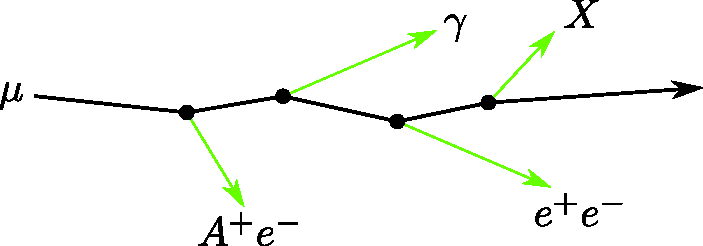
\includegraphics[height=0.5\textheight]{plots/muon_path.pdf}}

\usepackage{color}
\newcommand{\Hilight}{\makebox[0pt][l]{\color{tugreen}\rule[-4pt]{0.65\linewidth}{14pt}}}

\begin{document}



%%% TITLE

\begin{frame}
  \maketitle
\end{frame}

%%% Content

\begin{frame}{Inhalt}
   \begin{columns}
       \begin{column}{0.4\textwidth}
            \begin{block}{1. Einführung in PROPOSAL}
              \centering
                \vspace{2mm}
              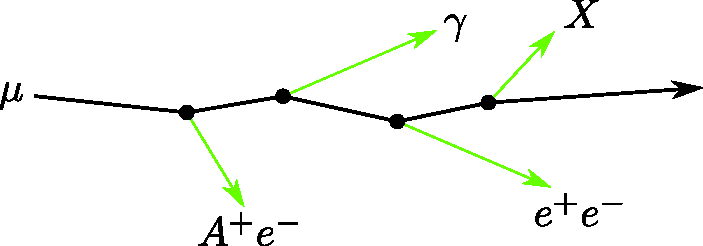
\includegraphics[height=0.15\textheight]{plots/muon_path.pdf}
                \vspace{2mm}
            \end{block}
       \end{column}
       \begin{column}{0.4\textwidth}
            \begin{block}{2. Seltene Prozesse}
 
            \end{block}
       \end{column}
   \end{columns}
   \begin{columns}
       \begin{column}{0.4\textwidth}
            \begin{block}{3. Schauerpropagation}
            \end{block}
       \end{column}
       \begin{column}{0.4\textwidth}
           \begin{block}{4. Ergebnisse}
              \centering
                \vspace{2mm}
              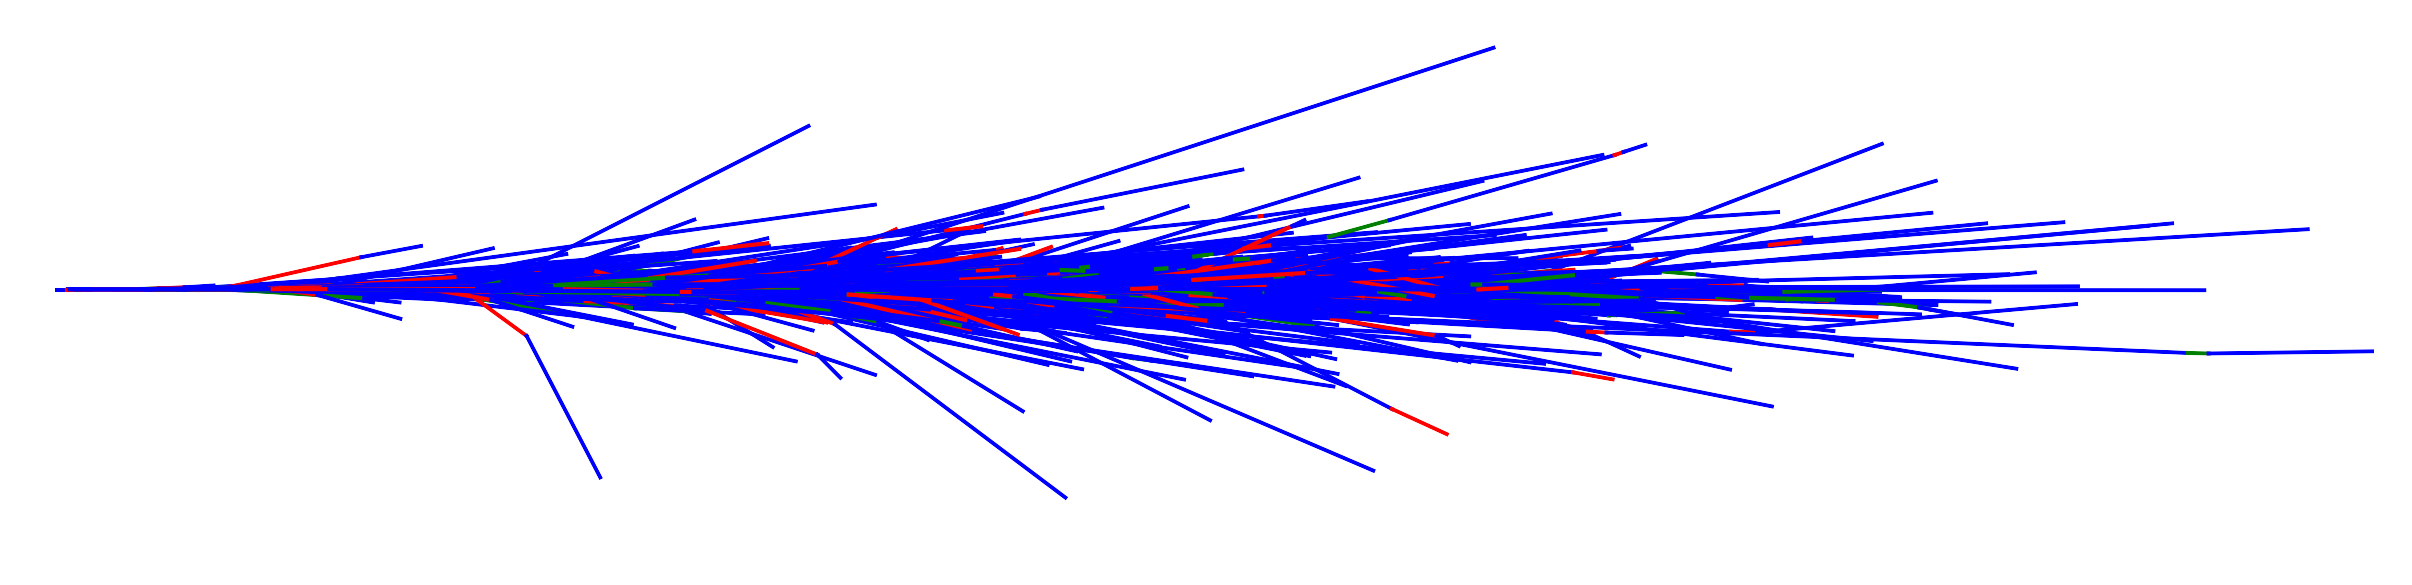
\includegraphics[height=0.15\textheight]{plots/shower_nolegend.png}
                \vspace{2mm}
           \end{block}
       \end{column}
   \end{columns}
\end{frame}

%%% 1. Einführung in PROPOSAL

\begin{frame}
      \begin{aquote}{"Der Leptonpropagator PROPOSAL" - Dissertation von Jan-Hendrik Köhne}
      Ziel ist es ein Monte-Carlo Programm zu entwickeln, welches einerseits die bei der \textcolor{red}{Propagation von Leptonen} auftauchende große Anzahl an Wechselwirkungen (einige tausend)
      mit \textcolor{red}{großer Genauigkeit} beschreibt und andererseits den \textcolor{red}{algorithmischen Fehler} so gering wie möglich hält. 
      \end{aquote}
\end{frame}


\begin{frame}
  \Huge
  \begin{align*}
      \frac{\mathrm{d}\sigma}{\mathrm{d}v} \quad \underbrace{\longrightarrow}_{?} \quad \text{Energieverluste}
  \end{align*}\\[1cm]
  \large
  \centering
  mit $v$ dem relativen Energieverlust eines Primärteilchens
\end{frame}



\begin{frame}
  \huge
  \begin{align*}
      \underset{\text{stochastische Verluste}}{v > v_\text{cut}} &&  \underset{\text{kontinuierliche Verluste}}{v < v_\text{cut}}
  \end{align*}\\
  \vspace{20px}
    \Large
    \centering
  mit $v_\text{cut} = \text{min}\left[\sfrac{e_\text{cut}}{E}, v\prime_\text{cut} \right]$
\end{frame}

%%% 2. Seltene Prozesse

%%% 3. Schauerpropagation

%%% 4. Ergebnisse


%%% End

\begin{frame}[t]
  \vspace{-5mm}
  \begin{minipage}[t][0.8\textheight][t]{\textwidth}
      \begin{columns}
    \column{0.5\textwidth}
      \begin{figure}
          \centering
          
\includegraphics[width=0.6\linewidth]{plots/github.pdf}
           \captionsetup{format=myformat}
          \caption*{https://github.com/tudo-\\astroparticlephysics/PROPOSAL}
      \end{figure}
    \column{0.5\textwidth}
      \begin{figure}
          \centering
          
\includegraphics[width=0.6\linewidth]{plots/arxiv.pdf}
          \captionsetup{format=myformat}
          \caption*{https://arxiv.org/abs/1809.07740 \\ \phantom{astroparticlephysics/PROPOSAL}}
      \end{figure}
  \end{columns}
  \end{minipage}
  \vfill
  \begin{minipage}{\textwidth}
      \smaller
      \begin{center}
      PROPOSAL may be modified and distrubuted under terms of a modified LGPL license.\\More information on our GitHub page.
      \end{center}
  \end{minipage}
\end{frame}
\end{document}
